\documentclass[12pt, varwidth, border=5mm]{standalone}
\usepackage{tikz}
\usepackage{amsmath}
% Underlining package
\usepackage{ulem}
\usetikzlibrary{calc}
\usetikzlibrary{angles,quotes}
\usetikzlibrary{decorations.markings, arrows.meta}
% \usepackage[a4paper, portrait, margin=1cm]{geometry}

\begin{document}
\section*{ }
    \begin{minipage}{0.55\textwidth}
  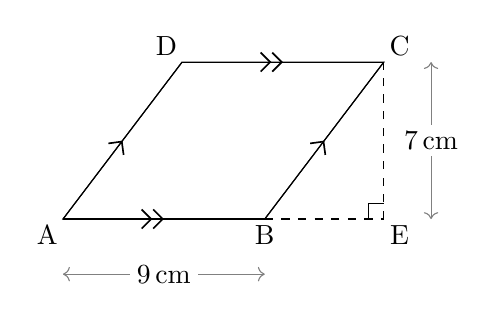
\begin{tikzpicture}[scale=1.0, baseline=(current bounding box.north)]
    \begin{scope}[rotate=0]

        \coordinate (A) at (0,0);
        \coordinate (B) at (2.562,0);
        \coordinate (E) at ($(B)+(1.512,0)$);  % extend out
        \coordinate (C) at ($(B)+(1.512,1.993)$); % Perpendicular upwards
        \coordinate (D) at ($(A)+(1.512,1.993)$); % Perpendicular upwards

        \draw (A)--(B)--(C)--(D)--cycle;
        \draw[dashed] (B)--(E);
        \draw[dashed] (E)--(C);

        \pic [draw, -, angle radius=0.2cm] {right angle=B--E--C};

        \draw[>=Straight Barb, postaction={decorate}, decoration={markings, mark=at position 0.5 with {\arrow[scale=1.5]{>>}}}] (A)--(B);
        \draw[>=Straight Barb, postaction={decorate}, decoration={markings, mark=at position 0.5 with {\arrow[scale=1.5]{>>}}}] (D)--(C);
        \draw[>=Straight Barb, postaction={decorate}, decoration={markings, mark=at position 0.5 with {\arrow[scale=1.5]{>}}}] (B)--(C);
        \draw[>=Straight Barb, postaction={decorate}, decoration={markings, mark=at position 0.5 with {\arrow[scale=1.5]{>}}}] (A)--(D);



        % Vertex LABELS
        % Labels relative to shape geometry
        \node at ($(A)+(-0.2,-0.2)$) {A};
        \node at ($(B)+(0.0,-0.2)$) {B};
        \node at ($(E)+(0.2,-0.2)$) {E};
        \node at ($(C)+(0.2,0.2)$) {C};
        \node at ($(D)+(-0.2,0.2)$) {D};


        % dotted/dashed arrows shifted away from edges
        % Horizontal side (A-B), shifted down yshift=0mm,
        \draw[<->, gray]
            ($(A) + (0,-0.7cm)$) -- ($(B) + (0,-0.7cm)$)
            node[black, midway, fill=white, inner sep=2.5pt] {9\,cm};

        % Vertical side (D-C), shifted right xshift=0mm,
        \draw[<->, gray]
            ($(E)+(0.6,0)$) -- ($(E |- C)+(0.6,0)$)
            node[black, midway, fill=white, inner sep=2.5pt] {7\,cm};

    \end{scope}
\end{tikzpicture}
\end{minipage}%
\hfill
\begin{minipage}{.4\textwidth}
  \begin{align*}
    \text{Area} &= \text{bh} \\
    \text{Area} &= 9 \text{cm} \times 7 \text{cm}  \\
    \text{Area} &= 63 \text{cm}^2
  \end{align*}
\end{minipage}

\end{document}
